%&../settings/preamble.main

\ifsubfile
\pagestyle{plain}
\setcounter{chapter}{8}

% arara: pdflatex: { options: ["--output-directory=../build"], draft: yes, synctex: no }
% arara: pdflatex: { options: ["--output-directory=../build"], synctex: no }
\begin{document}
\fi
\chapter{Grafi}

\section{Introduzione}

Un grafo non è altro che un insieme di entità collegate da un insieme di relazioni che possono essere interpretate in vari modi.

Il questa parte della lezione affronteremo i problemi che possono essere risolti tramite grafi non pesati, ossia:
\begin{itemize}
	\item ricerca del cammino più breve, misurato in numero di archi (che differisce dal problema del cammino minimo definito su grafi pesati che cerca di stabilire quale sia il cammino meno costoso);
	\item componenti (fortemente) connesse;
	\item verifica ciclicità;
	\item ordinamento topologico.
\end{itemize}

\begin{comment}
\subsection{Esempi}

Moltissimi problemi possono essere visti come problemi su grafi.
Sebbene i problemi abbiano forma astratta, le loro applicazioni si trovano poi negli ambiti più disparati.
Ad esempio:
\begin{itemize}
	\item Quando cercate qualcuno su LinkedIn, vi restituisce un \enquote{grado di conoscenza};
	\item L'ordinamento topologico viene utilizzato per stabilire un ordine di azioni in un grafo di dipendenze;
	\item Gli algoritmi di model checking utilizzati per la verifica formale del software sono basati sull'identificazione delle componenti fortemente connesse.
\end{itemize}

Dalle testimonianze otteniamo il grafo degli incontri, ma abbiamo bisogno di ragionare sul grafo degl intervalli.
\end{comment}

\subsection{Definizioni}

\begin{definition}[Grafo orientato, \foreign{directed}]
	Un grafo orientato è una coppia \(G = (V,E)\) dove \(V\) è un insieme di nodi (node) o vertici (vertex), mentre \(E\) è un insieme di coppie ordinate \((u, v)\) di nodi detti archi (edges).
\end{definition}

\begin{definition}[Grafo non orientato, \foreign{undirected}]
	Un grafo non orientato è una coppia \(G = (V,E)\) dove è un insieme di nodi (node) o vertici (vertex), mentre \(E\) è un insieme di coppie \alert{non ordinate} \((u, v)\) dette archi (edges).
\end{definition}

\begin{figure}[H]
	\begin{subfigure}{.5\textwidth}\centering
		% 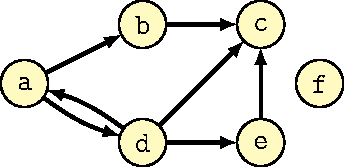
\includegraphics{definition-directed}
		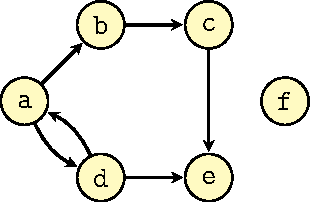
\includegraphics{rev-graph-directed}
		\caption{Grafo diretto}
	\end{subfigure}\hfill
	\begin{subfigure}{.5\textwidth}\centering
		% 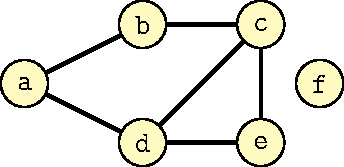
\includegraphics{definition-undirected}
		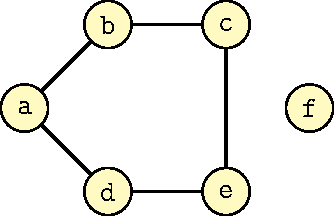
\includegraphics{rev-graph-undirected}
		\caption{Grafo indiretto}
	\end{subfigure}
\end{figure}

\subsection{Terminologia}

\begin{property*}[Adiacenza]
	Un vertice \(v\) è detto \alert{adiacente} a \(u\) se esiste un arco \((u,v)\).
\end{property*}

\begin{property*}[Incidenza]
	Un arco \((u,v)\) è detto \alert{incidente} da \(u\) a \(v\).
\end{property*}

\clearpage
\begin{multicols}{2}
\centering
% 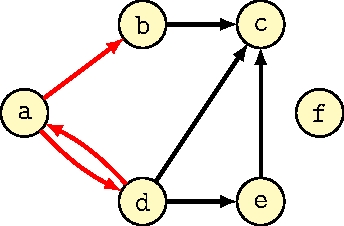
\includegraphics{adjacent}
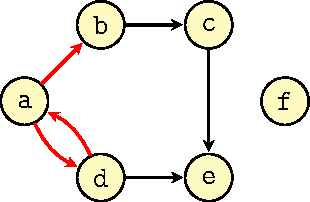
\includegraphics{rev-graph-directed-adj}
\columnbreak
\begin{itemize}
	\item \((a,b)\) è incidente da \(a\) a \(b\)
	\item \((a,d)\) è incidente da \(a\) a \(d\)
	\item \((d,a)\) è incidente da \(d\) a a
	\item \(b\) è adiacente ad \(a\)
	\item \(d\) è adiacente ad \(a\)
	\item \(a\) è adiacente a \(d\)
\end{itemize}
\end{multicols}

\begin{note}
	In un grafo non orientato, la relazione di adiacenza è simmetrica.
\end{note}

\subsection{Ragionamenti sulla complessità}

Definiamo il numero di nodi con \(n = \abs{V}\), ed il numero di archi con \(m = \abs{E}\).
C'è una relazione precisa fra \(n\) ed \(m\). In un grafo non orientato \(m \leqslant \frac{n(n-1)}{2} = \Omicron(n^2)\), mentre in un grafo orientato \( m \leqslant n^2 - n = \Omicron(n^2)\).
Questi ordini di grandezza ci serviranno a valutare quale algoritmo utilizzare in base al numero di possibili archi.
La complessità viene quindi espressa in termini sia di \(n\) che di \(m\), ad esempio \(\Omicron(n+m)\).

\subsection{Casi speciali}

\subsection*{Completezza di un grafo}

Un grafo con un arco fra tutte le coppie di nodi è detto \emph{completo}.
Informalmente (non c'è accordo sulla definizione) parleremo di:
\begin{itemize}
	\item grafo \emph{sparso} se ha \enquote{pochi archi}; ad esempio grafi con \(m\) pari a \(\Omicron(n)\) o \(\Omicron(n \log n)\) sono considerati tali;
	\item grafo \emph{denso} se ha \enquote{tanti archi}; ad esempio grafi con \(m\) pari a \(\Omega(n^2)\).
\end{itemize}

\begin{figure}[H]
	\begin{subfigure}{.5\textwidth}\centering
		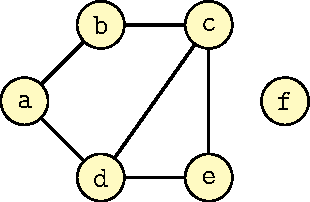
\includegraphics{rev-graph-undirected-sparse}
		\caption{Grafo sparso}
	\end{subfigure}\hfill
	\begin{subfigure}{.5\textwidth}\centering
		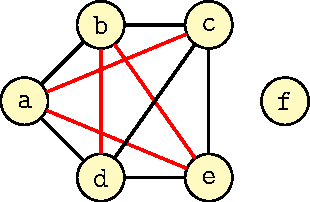
\includegraphics{rev-graph-undirected-dense}
		\caption{Grafo denso}
	\end{subfigure}
\end{figure}

\subsection*{Alberi radicati}

\begin{definition}[Albero non radicato, libero]
	Un albero libero (free tree) è un grafo connesso con \(m = n-1\), dove non viene identificata una radice.
\end{definition}

\begin{definition}[Albero radicato]
	Un albero radicato (rooted tree) è un grafo connesso con \(m = n-1\) nel quale uno dei nodi è designato come radice.
\end{definition}

\begin{definition}[Foresta]
	Un insieme di alberi è un grafo detto foresta.
\end{definition}

\begin{figure}[H]
	\begin{subfigure}{.5\textwidth}\centering
		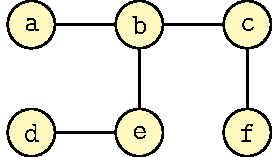
\includegraphics[page=1]{rev-forest}
		\caption{Albero libero}
	\end{subfigure}\hfill
	\begin{subfigure}{.5\textwidth}\centering
		\includegraphics[page=2]{rev-forest}
		\caption{Albero radicato}
	\end{subfigure}
\end{figure}

\subsection*{Definizioni}

\begin{definition}[Grado, \foreign{degree}]
	In un grafo non orientato il grado di un nodo è il numero di archi incidenti su di esso.
\end{definition}

\begin{definition}[Grado entrante, \foreign{in-degree}]
	In un grafo orientato il grado entrante di un nodo è il numero di archi entranti su di esso.
\end{definition}

\begin{definition}[Grado uscente, \foreign{out-degree}]
	In un grafo orientato il grado uscente di un nodo è il numero di archi uscenti da esso.
\end{definition}

\begin{figure}[H]
	\begin{subfigure}[t]{.5\textwidth}\centering
		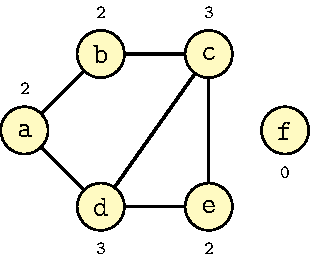
\includegraphics{rev-graph-undirected-degree}
		\caption{Grado di un grafo indiretto}
	\end{subfigure}\hfill
	\begin{subfigure}[t]{.5\textwidth}\centering
		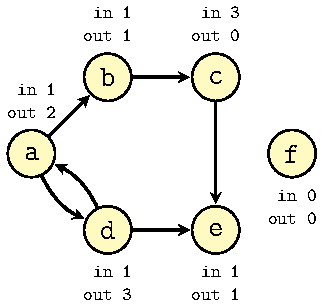
\includegraphics{rev-graph-directed-degree}
		\caption{Grado di un grafo diretto}
	\end{subfigure}
\end{figure}

% NB rispetto gli anni precedenti manca la definizione di catena?
\begin{definition}[Cammino, \foreign{path}]
	In un grafo \(G = (V,E)\), un cammino \(C\) di lunghezza \(k\) è una sequenza di nodi \(u_1, \dots, u_k\) tale che \((u_i, u_{i+1}) \in E\) per \(0 \leqslant i \leqslant k-1 \).
\end{definition}

\begin{figure}[H]\centering
	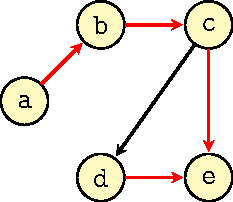
\includegraphics{rev-graph-directed-path}
	\caption[Cammino in un grafo diretto]{Cammino in un grafo diretto, \(a, b, c, e, d\) è un cammino di lunghezza \(4\)}
\end{figure}

\begin{note}
Un cammino è detto semplice se tutti i suoi nodi sono distinti.
\end{note}

\clearpage
\subsection{Specifica}

Nella versione più generale, il grafo è una struttura di dati dinamica che permette di aggiungere e  rimuovere nodi e archi.
La specifica che utilizzeremo non prevede la rimozione dei nodi dal grafo.

\begin{algorithm}[H]
	\caption{Specifica della struttura dati \textsc{Graph}}
	%&../preamble

% arara: pdflatex: { synctex: no }
% arara: latexmk: { clean: partial }
\ifstandalone
\begin{document}
\NoCaptionOfAlgo
\begin{algorithm}[H]
\caption{Struttura dati grafo}
\fi

% Il \Graph è una struttura dati dinamica che permette di aggiungere e rimuovere nodi ed archi.

\graphConstructor \Comment*[r]{crea un grafo vuoto}

\BlankLine
\Set \VV \Comment*[r]{restituisce l'insieme di tutti i nodi}
\Int \graphSize \Comment*[r]{restituisce il numero di nodi}

\BlankLine
\Set \adj{\Node u} \Comment*[r]{restituisce l'insieme di nodi adiacenti a \(u\)}

\BlankLine
\nodeInsert{\Node \(u\)}				\Comment*[r]{aggiunge il nodo \(u\) al grafo}
\nodeDelete{\Node \(u\)}				\Comment*[r]{rimuove il nodo \(u\) dal grafo}

\BlankLine
\edgeInsert{\Node \(u\), \Node \(v\)}	\Comment*[r]{aggiunge l'arco \((u,v)\) al grafo}
\edgeDelete{\Node \(u\), \Node \(v\)}	\Comment*[r]{rimuove l'arco \((u,v)\) dal grafo}

\ifstandalone
\end{algorithm}
\RestoreCaptionOfAlgo
\end{document}
\fi

\end{algorithm}

% NOTE in questa facciata ho ridotto lo spazio fra le sottosezioni per dare più fiato alle immagini
\subsection{Memorizzazione}

Esistono due diversi modi per memorizzare un grafo:
\begin{enumerate}
	\item \textbf{matrici di adiacenza}: utilizza una matrice contenente un bit per indicare la presenza di ciascun arco: questo permette di controllare in tempo costante se un determinato arco è presente.
	La matrice di adiacenza viene ottenuta nel seguente modo:
	\[
		m_{uv} =
		\begin{dcases}
			1 & (u,v) \in E \\
			0 & (u,v) \not\in E
		\end{dcases}
	\]
	\item \textbf{lista di adiacenza}: una lista delle adiacenze presenti fra i nodi.
\end{enumerate}

\clearpage
\subsection*{Grafo orientato}
\vspace{-5pt}

Memorizzare un grafo orientato attraverso matrice di adiacenza occupa uno spazio pari a \(n^2\) bit, mentre se si utilizza una lista di adiacenza vengono occupati \(an + bm\) bit.

% NOTE ho rimosso il vettore di adiacenza per allineare le figure con le altre immagini
\begin{figure}[H]\hfill
	\begin{subfigure}[t]{.25\textwidth}\centering
		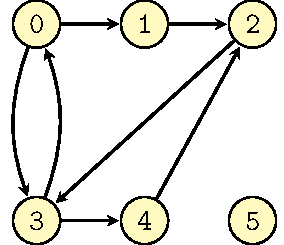
\includegraphics[width=\linewidth, height=3.5cm, keepaspectratio, page=1]{rev-memory-graph-directed}
		\caption{Grafo orientato}
	\end{subfigure}\hfill
	\begin{subfigure}[t]{.25\textwidth}\centering
		\includegraphics[width=\linewidth, height=3.5cm, keepaspectratio, page=2]{rev-memory-graph-directed}
		\caption{Matrice di adiacenza}
	\end{subfigure}\hfill
	\begin{subfigure}[t]{.35\textwidth}\raggedright
		\includegraphics[width=\linewidth, height=3.5cm, keepaspectratio, page=3]{rev-memory-graph-directed}
		\caption{Lista di adiacenza}
	\end{subfigure}%\hfill
	% \begin{subfigure}[t]{.15\textwidth}\raggedright
	% 	\includegraphics[width=\linewidth, height=3cm, keepaspectratio, page=4]{rev-memory-graph-directed}
	% 	\caption{Vettore di adiacenza}
	% \end{subfigure}\hfill\null
\end{figure}

\vspace{-20pt}
\subsection*{Grafo non orientato}
\vspace{-5pt}

Se il grafo non è orientato ed utilizziamo una matrice di adiacenza per memorizzarlo, è sufficiente memorizzare solo la metà superiore, occupando uno spazio pari a \(n(n-1)/2\) bit, mentre con lista di adiacenza dobbiamo raddoppiare i puntatori occupando \(an + 2 \cdot bm\) bit.

\begin{figure}[H]\hfill
	\begin{subfigure}[t]{.25\textwidth}\centering
		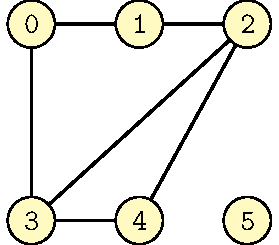
\includegraphics[width=\linewidth, height=3.5cm, keepaspectratio, page=1]{rev-memory-graph-undirected}
		\caption{Grafo non orientato}
	\end{subfigure}\hfill
	\begin{subfigure}[t]{.25\textwidth}\centering
		\includegraphics[width=\linewidth, height=3.5cm, keepaspectratio, page=2]{rev-memory-graph-undirected}
		\caption{Matrice di adiacenza}
	\end{subfigure}\hfill
	\begin{subfigure}[t]{.35\textwidth}\raggedright
		\includegraphics[width=\linewidth, height=3.5cm, keepaspectratio, page=3]{rev-memory-graph-undirected}
		\caption{Lista di adiacenza}
	\end{subfigure}
\end{figure}

\vspace{-20pt}
\subsection*{Grafo pesato}
\vspace{-5pt}

Infine se il grafo è pesato ed usiamo le matrici per rappresentarlo possiamo memorizzare il peso al posto del valore booleano, l'assenza dell'arco è quindi segnalata da un valore particolare (come \(-1\) o \(\infty\) in base alla procedura che vogliamo risolvere).
Mentre se utilizziamo una lista di adiacenza memorizzeremo semplicemente il peso.

\begin{figure}[H]\hfill
	\begin{subfigure}[t]{.25\textwidth}\centering
		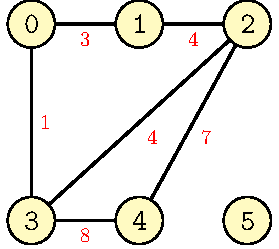
\includegraphics[width=\linewidth, height=3.5cm, keepaspectratio, page=1]{rev-memory-graph-weighted}
		\caption{Grafo pesato}
	\end{subfigure}\hfill
	\begin{subfigure}[t]{.25\textwidth}\centering
		\includegraphics[width=\linewidth, height=3.5cm, keepaspectratio, page=2]{rev-memory-graph-weighted}
		\caption{Matrice di adiacenza pesata}
	\end{subfigure}\hfill
	\begin{subfigure}[t]{.35\textwidth}\raggedright
		\includegraphics[width=\linewidth, height=3.5cm, keepaspectratio, page=3]{rev-memory-graph-weighted}
		\caption{Lista di adiacenza pesata}
	\end{subfigure}
\end{figure}

% TODO tabella implementazione nei vari linguaggi
% Noi utilizzeremo dei vettori idealmente statici o dinamici.

\clearpage
\subsection*{Dettagli sull'implementazione}

Nel seguito, se non diversamente specificato, assumeremo che:
\begin{itemize}
	\item l'implementazione sia basata su vettori di adiacenza (statici o dinamici);
	\item l'accesso alle informazioni abbia costo costante (ossia che la classe \Node sia \mbox{equivalente a \Int);}
	\item le operazioni per aggiungere nodi e archi abbiano costo ammortizzato \(\Omicron(1)\);
	\item dopo l'inizializzazione, il grafo sia statico.
\end{itemize}

% TODO importare codice implementazione pesata con dizionari in python
% TODO esempio di esecuzione

\subsection*{Iterazione su nodi e archi}

Negli algoritmi che seguiranno utilizzeremo questi schemi di codice per iterare su nodi ed archi.

\begin{algorithm}[H]
	\caption[Come iterare su nodi ed archi]{Schemi di iterazione per nodi ed archi}

	\BlankLine
	\tcp{iterare sui nodi}
	\ForEach{\(u \in G.\VV\)}{
		\{ \alert{Esegui operazioni sul nodo \(u\)} \}\;
	}

	\BlankLine
	\tcp{iterare sugli archi}
	\ForEach{\(u \in G.\VV\)}{
	\{ \textcolor{faded}{Esegui operazioni sul nodo \(u\)} \}\;

		\BlankLine
		\ForEach{\(v \in G.\adj{u}\)}{
			\{ \alert{Esegui operazioni sull'arco \(u, v\)} \}\;
		}
	}
\end{algorithm}

\paragraph{Complessità dell'iterazione}
Quest'operazione costa \(\Omicron(m+n)\) con le liste di adiacenza, mentre \(\Omicron(n^2)\) con le matrici di adiacenza.

\subsection*{Riassumendo}

Le matrici sono ideali per grafi \emph{densi}, occupano uno spazio \(\Omicron(n^2)\) e iterare su tutti gli archi costa \(\Omicron(n^2)\), verificare se \(u\) è adiacente a \(v\) richiede tempo costante \(\Omicron(1)\).

Le liste di adiacenza sono ideali per grafi \emph{sparsi}, occupano uno spazio \(\Omicron(n+m)\) e iterare su tutti gli archi costa \(\Omicron(n+m)\), verificare se \(u\) è adiacente a \(v\) richiede tempo lineare \(\Omicron(n)\).

\clearpage
\section{Visite dei grafi}

Dato un grafo \(G = (V,E)\) e un vertice \(r \in V\) di partenza (che prende il nome di \emph{radice} o di \emph{sorgente}), si vuole visitare una e una volta sola tutti i nodi del grafo che possono essere raggiunti da \(r\).

\paragraph{In ampiezza}
La visita in ampiezza effettua una visita dei nodi per livelli: prima visita la radice, poi i nodi a distanza uno dalla radice, poi i nodi a distanza due e così via\dots
Una possibile applicazione di questa visita è quella di calcolare i cammini più brevi da una singola sorgente.

\paragraph{In profondità}
La visita in profondità effettua una visita ricorsiva: per ogni nodo adiacente, si visita il nodo e tutti i suoi nodi adiacenti ricorsivamente.
Delle possibili applicazioni sono l'ordinamento topologico, la verifica della ciclicità e le componenti connesse e fortemente connesse.

\subsection{Visita in ampiezza}

Un approccio ingenuo alla visita di un grafo potrebbe essere il seguente:

\begin{algorithm}[H]
	\caption{Primo tentativo di visita di un grafo}
	\prototype{\visitaGrafo{\Graph \(G\)}}{
		\ForEach{\(u \in G.\VV\)}{
			\{ \alert{visita nodo \(u\)} \}\;
			\ForEach{\(v \in G.\adj{u}\)}{
				\{ \alert{visita arco \((u,v)\)} \}\;
			}
		}
	}
\end{algorithm}

Ma la struttura del grafo non viene presa in considerazione, poiché si itera su tutti i nodi e gli archi senza alcun criterio.
Un possibile approcio potrebbe essere quello di sfruttare l'algoritmo delle visite sugli alberi

\begin{algorithm}[H]
	\caption{Algoritmo adatto all'attraversamento degli alberi}
	%&../preamble

% arara: pdflatex: { synctex: no }
% arara: latexmk: { clean: partial }
\ifstandalone
\begin{document}
\begin{algorithm}[H]
\fi
\prototype{\visitaAlbero{\Graph \(G\), \Int \(r\)}}{

	\BlankLine
	\Queue \(Q\) \Assign \queueConstructor\;

	\(Q\).\queueInsert{\(r\)}\;

	\BlankLine
	\While{\Not \(Q\).\setEmpty}{
		\Node \(u\) \Assign \(Q\).\queueRemove\;

		\{ visita il nodo \(u\) \}\;

		\BlankLine
		\ForEach{\(u \in G.\adj{u}\)}{
			\(Q\).\queueInsert{\(v\)}\;
		}
	}
}
\ifstandalone
\end{algorithm}
\end{document}
\fi

\end{algorithm}

\clearpage
\begin{figure}[H]
	\centering

	\begin{subfigure}{.5\textwidth}
		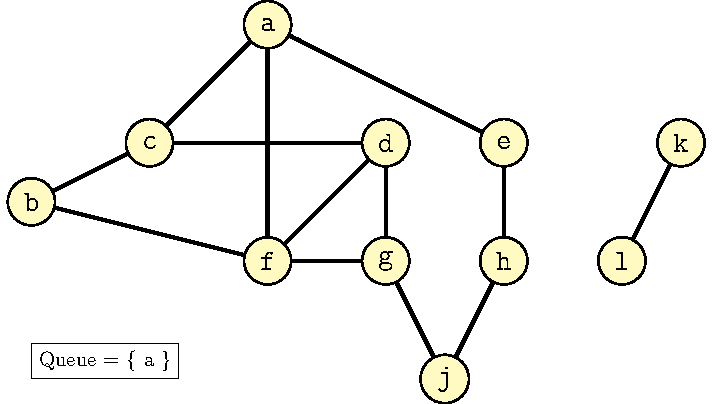
\includegraphics[width=\linewidth, page=1]{errata}
	\end{subfigure}\hfill
	\begin{subfigure}{.5\textwidth}
		\includegraphics[width=\linewidth, page=2]{errata}
	\end{subfigure}

	\begin{subfigure}{.5\textwidth}
		\includegraphics[width=\linewidth, page=3]{errata}
	\end{subfigure}\hfill
	\begin{subfigure}{.5\textwidth}
		\includegraphics[width=\linewidth, page=4]{errata}
	\end{subfigure}

	\caption{Esempio di attraversamento di un grafo\\tramite la procedura di visita di un albero}
\end{figure}

Dall'esempio possiamo notare come i nodi vengano reinseriti all'infinito all'interno della coda e questo non permette all'algoritmo di terminare.
Negli alberi, data la loro struttura, abbiamo la sicurezza che non visiteremo mai lo stesso nodo più di una volta.
Abbiamo bisogno di un meccanismo che ci permetta di evitare che questo avvenga.
Possiamo farlo memorizzando i nodi che abbiamo già visitato.

\begin{algorithm}[H]
	\caption{Algoritmo adatto all'attraversamento dei grafi}
	%&../preamble

% arara: pdflatex: { synctex: no }
% arara: latexmk: { clean: partial }
\ifstandalone
\begin{document}
\begin{algorithm}[H]
\fi
\prototype{\visitaGrafo{\Graph G, \Node r}}{

	\BlankLine
	\Set \(S\) \Assign \setConstructor \Comment*[l]{insieme generico, da specificare (\Stack, \Queue)}
	\(S.\setInsert{r}\) \Comment*[l]{inserisco il nodo, da specificare}

	\BlankLine
	\tcp{ho visitato il nodo}
	\{ \alert{marca il nodo \(r\) come \enquote{scoperto}} \}

	\BlankLine
	\tcp{fintanto che l'insieme non è vuoto}
	\While{\(S.\setSize > 0\)}{

		\BlankLine
		\tcp{la politica di rimozione dipende dal problema da risolvere}
		\Node \(u \Assign S.\setRemove\)\;

		\BlankLine
		\{ \alert{esamina il nodo \(u\)} \}

		\BlankLine
		\ForEach{\(v \in G.\adj{u}\)}{

			\BlankLine
			\{ \alert{esamina l'arco \((u,v)\)} \}

			\BlankLine
			\If{\(v\) non è già stato scoperto}{

				\BlankLine
				\tcp{serve a non inserire il nodo più di una volta}
				\{ \alert{marca il nodo \(v\) come \enquote{scoperto}} \}\;

				\(S.\setInsert{v}\) \Comment*[l]{inserisce il nodo nell'insieme, da specificare}
			}
		}
	}
}
\ifstandalone
\end{algorithm}
\end{document}
\fi

\end{algorithm}

\clearpage
Gli obiettivi della visita in ampiezza sono:
\begin{itemize}
	\item visitare i nodi a distanze crescenti dalla sorgente: visitare quindi i nodi a distanza \(k\) prima di quelli a distanza \(k+1\);
	\item calcolare il cammino più breve da \(r\) a tutti gli altri nodi, dove il cammino più breve è il percorso con il minor numero di archi;
	\item generare un albero in ampiezza (\foreign{breadth-first}): l'albero in ampiezza è un albero contenente tutti i nodi raggiungibili da \(r\), tale per cui il cammino dalla radice \(r\) al nodo \(u\) nell'albero corrisponde al cammino più breve da \(r\) a \(u\) nel grafo.
\end{itemize}

\begin{algorithm}[H]
	\caption{Procedura specializzata per la visita in ampiezza di un grafo}
	%&../preamble

% arara: pdflatex: { synctex: no }
% arara: latexmk: { clean: partial }
\ifstandalone
\begin{document}
\begin{algorithm}[H]
\fi

\BlankLine
\tcp{visitare tutti i nodi a distanza \(k\) prima di visitare i nodi a distanza \(k+1\)}
\prototype{\bfsProc{\Graph \(G\), \Node \(r\)}}{
	\Queue \(S\) \Assign \queueConstructor \Comment*[l]{creo una pila}
	\(S\).\queueInsert{\(r\)} \Comment*[l]{inserisco la radice}

	\BlankLine
	\tcp{inizializzazione}
	\Array{\Bool} \(visitato\) \Assign \Array{\Bool}[1][G.n] \Comment*[l]{della dimensione del no.\ di nodi}
	\lForEach(\tcp*[h]{devo ancora visitarli}){\(u \in G.\VV - \{r\}\)}{
		\(visitato[u]\) \Assign \False
	}
	\(visitato[r]\) \Assign \True \Comment*[l]{radice visitata}

	\BlankLine
	\tcp{visita del grafo}
	\While{\Not \(S\).\setEmpty}{
		\Node \(u\) \Assign \(S\).\queueRemove \Comment*[l]{rimuovo un nodo}

		\BlankLine
		\{ \alert{esamina il nodo \(u\)} \}

		\BlankLine
		\ForEach(\tcp*[h]{per ciascun nodo adiacente "v"}){\(v \in G.\adj{u}\)}{

			\BlankLine
			\{ \alert{esamina l'arco \((u,v)\)} \}

			\BlankLine
			\If(\tcp*[h]{se non ho ancora visitato "v"}){\Not \(visitato[v]\)}{

				\BlankLine
				\(visitato[v]\) \Assign \True \Comment*[l]{marcalo come visitato}
				\(S.\queueInsert\) \Comment*[l]{inseriscilo nella coda}
			}
		}
	}
}
\ifstandalone
\end{algorithm}
\end{document}
\fi

\end{algorithm}

\clearpage
\subsection{Cammini più brevi}

Vediamo ora un'applicazione della visita in ampiezza: la ricerca dei cammini più brevi e lo facciamo tramite un esempio particolare: calcolare il numero di erd\"{o}s.

Paulo Erd\"{o}s è stato uno dei matematici più prolifici al mondo (1500+ articoli e 500+ co-autori).
Definiamo il numero di erdos nel seguente modo:
\begin{itemize}
	\item Erd\"{o}s ha valore \(erdos = 0\);
	\item i co-autori di Erd\"{o}s hanno \(erdos = 1\);
	\item se \(X\) è co-autore di qualcuno con \(erdos = k\) e non è co-autore con qualcuno con \(erdos < k\), allora \(X\) ha \(erdos = k+1\);
	\item le persone non raggiunte da questa definizione hanno \(erdos = +\infty\).
\end{itemize}

\begin{algorithm}[ht]
	% \caption{Visita in ampiezza (erdos)}
	\caption{Ricerca dei cammini minimi più brevi dalla radice}
	%&../preamble

% arara: pdflatex: { synctex: no }
% arara: latexmk: { clean: partial }
\ifstandalone
\begin{document}
\begin{algorithm}[H]
\fi

\BlankLine
\tcp{il camminimo più breve fra due vertici viene memorizzato tramite il vettore dei padri \(p\)}
\prototype{\erdos{\Graph \(G\), \Node \(r\), \Array{\Int} \(erdos\), \Node \(parent\)}}{

	\BlankLine
	\tcp{struttura di supporto}
	\Queue \(S\) \Assign \queueConstructor \Comment*[l]{creo una pila}
	\(S.\queueInsert{r}\) \Comment*[l]{inserisco la radice}

	\BlankLine
	\tcp{inizializzazione}

	\lForEach(\tcp*[h]{nodi non ancora raggiunti}){\(u \in G.\VV - \{r\}\)}{
		\(erdos[u]\) \Assign \(\infty\)
	}
	\(erdos[r]\) \Assign \True \Comment*[l]{erdõs ha distanza 0 da se stesso}
	\(parent[r]\) \Assign \Nil \Comment*[l]{per la stampa del cammino}

	\BlankLine
	\tcp{visita del grafo}
	\While{\Not \(S.\setEmpty\)}{
		\Node \(u\) \Assign \(S\).\queueRemove\;

		\BlankLine
		\ForEach{\(u \in G.\adj{u}\)}{

			\BlankLine
			\{ \alert{esamina l'arco \((u,v)\)} \}

			\BlankLine
			\If{\(erdos[v] \Equal \infty\)}{
				\tcp{il nodo non è stato ancora stato scoperto}

				\BlankLine
				\(erdos[v]\) \Assign \(erdos[u] + 1\) \Comment*[l]{gli assegno un livello di erdõs+1}
				\(parent[v]\) \Assign \(u\) \Comment*[l]{memorizzo il padre del nodo attuale nel v.\ dei padri}
				\(S\).\queueInsert{v} \Comment*[l]{è la prima volta che lo raggiungo quindi lo metto in coda}
			}
		}
	}
}
\ifstandalone
\end{algorithm}
\end{document}
\fi

\end{algorithm}

\clearpage
\begin{figure}[H]

	\begin{subfigure}[t]{.48\textwidth}
		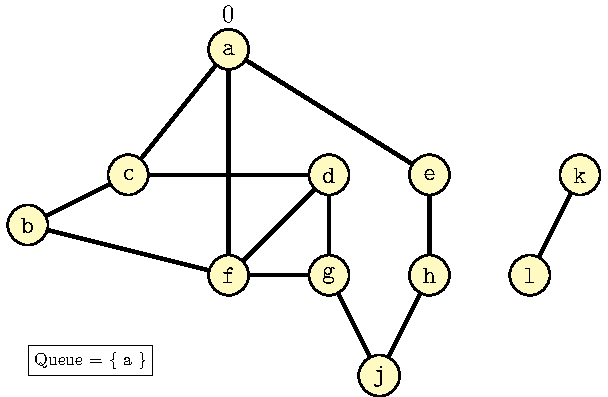
\includegraphics[width=\linewidth, page=1]{erd-rev}
		\caption{Assegno al nodo \(a\) distanza \(0\), lo aggiungo alla coda}
	\end{subfigure}\hfill
	\begin{subfigure}[t]{.48\textwidth}
		\includegraphics[width=\linewidth, page=2]{erd-rev}
		\caption{Estraggo il nodo \(a\),
			assegno ai suoi nodi adiacenti non ancora visitati (\(c\), \(f\), \(e\)) distanza \(a+1 = 1\)
			e li aggiungo alla coda}
	\end{subfigure}

	\begin{subfigure}[t]{.48\textwidth}
		\includegraphics[width=\linewidth, page=3]{erd-rev}
		\caption{Estraggo il nodo \(c\),
			assegno ai suoi nodi adiacenti non ancora visitati (\(b\), \(d\)) distanza \(c+1 = 2\)
			e li aggiungo alla coda}
	\end{subfigure}\hfill
	\begin{subfigure}[t]{.48\textwidth}
		\includegraphics[width=\linewidth, page=4]{erd-rev}
		\caption{Estraggo il nodo \(e\),
			assegno ai suoi nodi adiacenti non ancora visitati (\(h\)) distanza \(e+1 = 2\)\\
			e lo aggiungo alla coda}
	\end{subfigure}

	\begin{subfigure}[t]{.45\textwidth}
		% \addtocounter{subfigure}{4}
		\includegraphics[width=\linewidth, page=5]{erd-rev}
		\caption{Estraggo il nodo \(f\),
			assegno ai suoi nodi adiacenti non ancora visitati (\(b\), \(g\)) distanza \(f+1 = 2\)\\
			e li aggiungo alla coda}
	\end{subfigure}\hfill
	\begin{subfigure}[t]{.45\textwidth}
		\includegraphics[width=\linewidth, page=6]{erd-rev}
		\caption{Estraggo il nodo \(b\),
			il quale non ha nodi adiacenti non ancora visitati}
	\end{subfigure}

\end{figure}

\begin{figure}[H]

	\begin{subfigure}[t]{.45\textwidth}
		\addtocounter{subfigure}{6}
		\includegraphics[width=\linewidth, page=7]{erd-rev}
		\caption{Estraggo il nodo \(d\),
			il quale non ha nodi adiacenti non ancora visitati}
	\end{subfigure}\hfill
	\begin{subfigure}[t]{.45\textwidth}
		\includegraphics[width=\linewidth, page=8]{erd-rev}
		\caption{Estraggo il nodo \(h\),
			assegno al suo nodo adiacente non ancora visitato (\(j\)) distanza \(h+1 = 3\)\\
			e lo aggiungo alla coda}
	\end{subfigure}

	\begin{subfigure}[t]{.45\textwidth}
		\includegraphics[width=\linewidth, page=9]{erd-rev}
		\caption{Estraggo il nodo \(g\),
			il quale non ha nodi adiacenti non ancora visitati}
	\end{subfigure}\hfill
	\begin{subfigure}[t]{.45\textwidth}
		\includegraphics[width=\linewidth, page=10]{erd-rev}
		\caption{Estraggo il nodo \(j\),
			il quale non ha nodi adiacenti non ancora visitati}
	\end{subfigure}

	\begin{subfigure}[t]{.45\textwidth}
		\includegraphics[width=\linewidth, page=11]{erd-rev}
		\caption{Questo è l'albero risultante}
	\end{subfigure}\hfill
	\begin{subfigure}[t]{.45\textwidth}
		\includegraphics[width=\linewidth, page=12]{erd-rev}
		\caption{Rappresentazione dell'albero di copertura \textsf{bfs},
				 attraverso il vettore dei padri}
	\end{subfigure}

	\addtocounter{figure}{-1}
	\caption{Esempio di visita di un grafo\\tramite la procedura di visita in ampiezza}
\end{figure}

L'albero \enquote{di copertura} con radice \(r\) viene memorizzato tramite vettore dei padri (che nell'algoritmo di \erdos abbiamo chiamato \(parent\)).

\clearpage
\begin{algorithm}[H]
	\caption{Stampa del cammino}
	%&../preamble

% arara: pdflatex: { synctex: no }
% arara: latexmk: { clean: partial }
\ifstandalone
\begin{document}
\begin{algorithm}[H]
\fi

\BlankLine
\tcp{stampa il cammino da \(r\) a \(s\) nell'ordine corretto}
\prototype{\printPath{\Node \(r\), \Node \(s\), \Array{\Node} \(parent\)}}{
	\params{parent}[vettore dei padri]

	\BlankLine
	\uIf(\tcp*[h]{se è la radice}){\(r \Equal s\)}{
		\Print \(s\) \Comment*[l]{la stampo}
	}
	\uElseIf{\(parent[s] \Equal \Nil\)}{
		\Print \enquote{nessun cammino da \(r\) a \(s\)}
	}
	\Else{
		\tcp{la chiamata ricorsiva prima della stampa per stampare in ordine}
		\printPath{\(r\), \(parent[s]\), \(p\)}\;
		\Print \(s\)\;
	}
}

\ifstandalone
\end{algorithm}
\end{document}
\fi

\end{algorithm}

\subsection{Complessità della visita in ampiezza}

Ognuno degli \(n\) nodi viene inserito nella coda al massimo una volta, ed ogni volta che un nodo viene estratto tutti i suoi archi vengono analizzati una volta sola, per una complessità totale di \(\Omicron(m+n)\).
Il numero di archi analizzati è quindi
\[
	m = \sum_{u \in V} \mathit{out}_d(u)
\]
dove \(\mathit{out}_d(u)\) è il grado uscente (\foreign{out-degree}) del nodo \(u\).

% TODO aggiungere esercizi d'esame nella quale la soluzione richiede una visita in ampiezza

\subsection{Visita in profondità}

Molto spesso la visita in profondità è solo una parte di una soluzione ad un altro problema, viene utilizzata per esplorare un intero grafo, e non solo i nodi raggiungibili da una singola sorgente.

L'output dell'algoritmo non è più un singolo albero, ma una foresta \foreign{depth-first} (ossia un insieme di alberi \foreign{depth-first}).

La struttura dati utilizzata non è più una coda, bensì uno \foreign{stack} implicito (attraverso la ricorsione) o esplicito (vedremo un algoritmo nel seguito).

\begin{algorithm}[H]
	\caption{Visita in profondità, ricorsiva con stack implicito}
	%&../preamble

% arara: pdflatex: { synctex: no }
% arara: latexmk: { clean: partial }
\ifstandalone
\begin{document}
\begin{algorithm}[H]
\fi

\BlankLine
\tcp{genera un albero depth-first}
\prototype{\dfsProc{\Graph G, \Node u, \Array{\Bool} visitato}}{
	\(visitato[u] = \True\) \Comment*[l]{ho visitato il nodo}

	\BlankLine
	\lnl{dfs:pre-visita}%
	\{ \alert{esamina il nodo \(u\) (caso \emph{pre}-visita)} \}

	\BlankLine
	\ForEach{\(v \in G.\adj{u}\)}{

		\BlankLine
		\{ \alert{esamina l'arco \((u,v)\)} \}

		\BlankLine
		\If(\tcp*[h]{se non l'ho ancora visitato}){\Not \(visitato[v]\)}{
			\tcp{chiamata ricorsiva}
			\dfsProc{G, v, visitato} \Comment*[l]{lo visito ricorsivamente}
		}
	}

	\BlankLine
	\lnl{dfs:post-visita}%
	\{ \alert{esamina il nodo \(u\) (caso \emph{post}-visita)} \}
}

\ifstandalone
\end{algorithm}
\end{document}
\fi

\end{algorithm}

\paragraph{Analisi della complessità}
Questo algoritmo ha la stessa complessità della visita in ampiezza: \(\Omicron(n+m)\) con il grafo implementato tramite liste di adiacenza, e \(\Omicron(n^2)\) con matrice di adiacenza.

Si presenta però un problema, mentre con gli alberi possiamo assumere che la loro profondità sia limitata, con i grafi non possiamo fare lo stesso discorso.
Eseguire una visita in profondità basata su chiamate ricorsive può essere rischioso (errore di \textsf{stack overflow}) in grafi molto grandi e connessi (in particolare se non sono orientati, in quanto la visita analizza tutti i nodi).
\`{E} possibile che la profondità raggiunta sia troppo grande per la dimensione dello stack del linguaggio.
In tali casi, si preferisce utilizzare una visita in ampiezza, oppure in profondità ma basata su stack esplicito.

\begin{algorithm}[H]
	\caption[Visita in profondità iterativa]{Visita in profondità, iterativa con stack esplicito, visita in \emph{pre}-ordine}
	%&../preamble

% arara: pdflatex: { synctex: no }
% arara: latexmk: { clean: partial }
\ifstandalone
\begin{document}
\algorithmstyle{ruled}
\NoCaptionOfAlgo
\begin{algorithm}[H]
\caption[Visita in profondità iterativa]{Visita in profondità, iterativa con stack esplicito e visita in \emph{pre}-ordine}
\fi

\BlankLine
\tcp{effettua una visita in profondità iterativa}
\prototype{\dfsProcIter{\Graph G, \Node r}}{
	\Stack \(S \Assign \stackConstructor\)\;
	\(S.\stackPush{r}\) \Comment*[l]{inserisco la radice nella pila}

	\BlankLine
	\Array{\Bool} \(visitato \Assign\) \new \Array{\Bool}[1][G.\graphSize]\;
	\lForEach{\(u \in G.\VV - \{r\}\)}{
		\(visitato[u] \Assign \False\)\;
	}
	\(visitato[r] \Assign \True\) \Comment*[l]{marco la radice come visitata}

	\BlankLine
	\While{\Not \(S.\stackEmpty\)}{

		\BlankLine
		\Node \(u \Assign S.\stackPop\) \Comment*[l]{estraggo un nodo}
		\If(\tcp*[h]{se non l'ho ancora visitato}){\Not \(visitato[v]\)}{
			\BlankLine
			\{ \alert{esamina il nodo \(u\) in \emph{pre}-ordine} \}\;
			\(visitato[v] \Assign \True\) \Comment*[l]{lo segno come visitato}

			\BlankLine
			\ForEach(\tcp*[h]{per ciascun nodo adiacente}){\(v \in G.\adj{u}\)}{

				\BlankLine
				\{ \alert{esamina l'arco \((u,v)\)} \}

					\(S.\stackPush{v}\) \Comment*[l]{lo inserisco nella pila}
			}
		}
	}
}

\ifstandalone
\end{algorithm}
\RestoreCaptionOfAlgo
\algorithmstyle{tworuled}
\end{document}
\fi

\end{algorithm}

La procedura si ottiene semplicemente sostituendo una pila alla coda utilizzata nella visita in ampiezza.

Un nodo può essere inserito nella pila più volte (tante volte quanti sono gli archi entranti in quel nodo, il numero di archi entranti in tutti i nodi è limitato superiormente dal numero di archi \(m\), quindi \(\Omicron(m)\), in quanto il controllo se un nodo è già stato inserito viene fatto all'estrazione, non all'inserimento come avveniva in precedenza.

\paragraph{Complessità della visita in ampiezza con stack esplicito}
Inserimenti ed estrazioni sono pari al numero degli archi, quindi \(\Omicron(m)\), visitare gli archi costa \(\Omicron(m)\) e le visite dei nodi costano \(\Omicron(n)\), per una complessità risultante di \(\Omicron(m+n)\), invariata rispetto agli algoritmi precedenti.

\paragraph{Visita in post-ordine}
\`{E} possibile effettuare una visita in profondità con una procedura con stack esplicito e visita in \emph{post}-ordine ma abbiamo bisogno di aggiungere due \enquote{flag}: \textsf{discovery} e \textsf{finish}.

Quando un nodo viene scoperto viene inserito nello stack con il tag \textsf{discovery};
quando un nodo viene estratto dalla coda con tag \textsf{discovery}: viene re-inserito con il tag \textsf{finish} e tutti i suoi vicini vengono inseriti;
Quando un nodo viene estratto dalla coda con tag \textsf{finish}, viene effettuata la post-visita.
Non vedremo il codice poiché è complicato e i dettagli non sono interessanti.

% TODO mettere esercizio dove questo avviene

\clearpage
\subsection{Componenti connesse}

Vogliamo identificare le componenti connesse di un grafo.
Prima di tutto vogliamo capire se è connesso, dopodiché vogliamo sapere quante sono le sue componenti connesse.
Il motivo per cui vogliamo farlo è che molti algoritmi che operano sui grafi iniziano decomponendo il grafo nelle sue componenti connesse per poi ri-comporre i risultati assieme.
Sono definite due tipologie di problemi:
\begin{itemize}
	\item componenti connesse (\foreign{Connected Components, CC});
	\item componenti fortemente connesse (\foreign{Strongly Connected Components, SCC})
\end{itemize}
Entrambi i problemi sono definiti su grafi non orientati.

Per capire meglio il problema abbiamo bisogno di qualche definizione:
\begin{definition}[Raggiungibilità di un nodo]
	Un nodo \(v\) è raggiungibile da un nodo \(u\) se esiste almeno un cammino da \(u\) a \(v\).
\end{definition}

% Un nodo \(d\) è raggiungibile dal nodo \(a\) e viceversa.
% Un nodo \(d\) è raggiungibile dal nodo \(a\), ma non viceversa.
% TODO esempio di raggiungibilità 50/101

\begin{definition}[Grafo non orientato connesso]
	Un grafo non orientato \(G = (V, E)\) è connesso se e solo se ogni suo nodo è raggiungibile da ogni altro suo nodo.
\end{definition}

% TODO inserire esempio di grafo connesso e non connesso

\begin{definition}[Componente connessa]
	Un grafo \(G' = (V', E')\) è una componente connessa di \(G\) se e solo se \(G'\) è un sottografo connesso e massimale di \(G\).
\end{definition}

\begin{definition}[Sottografo]
	\(G'\) è un sottografo di \(G\) \((G' \subseteq G) \Leftrightarrow V' \subseteq V\) e \(E' \subseteq E\)
\end{definition}

\begin{definition}[Grafo massimale]
	\(G'\) è massimale se e solo se non esiste nessun altro sottografo \(G''\) di \(G\) tale che \(G''\) è connesso e più grande di \(G'\) (ad esempio \(G' \subseteq G'' \subseteq G\))
\end{definition}

% TODO produrre esempio di sottografo ma non massimale e di sottografo massimale

Vogliamo quindi verificare se un grafo è connesso oppure no, ed identificare le sue componenti connesse.
Per farlo utilizzeremo di un vettore (che chiameremo \(id\)), il quale conterrà l'indentificatore alla quale la componente appartiene (\(id[u]\) è l'indentificatore della c.c.\ a cui appartiene \(u\)).
Un grafo risulta connesso se, al termine della visita in profondità, tutti i suoi nodi risultano marcati.
Altrimenti la visita deve ricominciare da capo da un nodo non marcato, identificando una nuova componente.

\begin{algorithm}[H]
	\caption[Componenti Connesse]{Identifica le componenti connesse di un grafo non orientato}
	%&../preamble

% arara: pdflatex: { synctex: no }
% arara: latexmk: { clean: partial }
\ifstandalone
\begin{document}
\begin{algorithm}[H]
\fi

\BlankLine
% \tcp{identifica le componenti connesse di un grafo non orientato}
\tcp{parte iterativa}
\prototype{\Array{\Int} \ConnectedComponents{\Graph G, \Stack S}}{

	\BlankLine
	\tcp{creo un vettore della dimensione dei nodi del grafo}
	\Array{\Int} \(id\) \Assign \new \Array{\Int}[1][G.\setSize]\;
	\tcp{inizializzo il vettore}
	\lForEach{\(u \in G.\VV\)}{
		\(id[u] \Assign 0\)
	}

	\Int \(counter = 0\) \Comment*[l]{contatore delle componenti connesse}

	\BlankLine
	\ForEach(\tcp*[h]{per ogni nodo del grafo}){\(u \in G.\VV\)}{

		\BlankLine
		\If(\tcp*[h]{ho trovato una nuova componente connessa}){\(id[u] \Equal 0\)}{
			\Increment{counter} \Comment*[l]{aggiorno il contatore}

			\BlankLine
			\tcp{effettuo una chiamata ricorsiva sul nodo scoperto}
			\ccdfs{G, counter, u, id}
		}
	}

	\BlankLine
	\tcp{restituisco l'identificativo della componente connessa}
	\Return \(id\)
}
\ifstandalone
\end{algorithm}
\end{document}
\fi

	%&../preamble

% arara: pdflatex: { synctex: no }
% arara: latexmk: { clean: partial }
\ifstandalone
\begin{document}
\begin{algorithm}[H]
\fi

\BlankLine
\tcp{visita ricorsiva di ciascuna componente}
\prototype{\ccdfs{\Graph G, \Int counter, \Node u, \Array{\Int} id}}{

	\vspace{2pt}
	\params{counter}[identificatore di quante cc ho trovato fin'ora]
	\params{u}[il nodo che sto visitando]
	\params{id}[l'identificativo della componente]

	\BlankLine
	\tcp{memorizzo l'identificativo della cc}
	\(id[v] \Assign counter\)\;

	\BlankLine
	\ForEach(\tcp*[h]{per ciascun nodo adiacente}){\(v \in G.\adj{u}\)}{

		\BlankLine
		\If(\tcp*[h]{non è ancora stato visitato}){\(id[v] \Equal 0\)}{
			\tcp{\(v\): il nodo su cui vado ad operare}

			\BlankLine
			\ccdfs{G, counter, v, id} \Comment*[l]{lo visito ricorsivamente}
		}
	}
}
\ifstandalone
\end{algorithm}
\end{document}
\fi

\end{algorithm}

\clearpage
\begin{figure}[p]

	\begin{subfigure}[t]{.48\textwidth}
		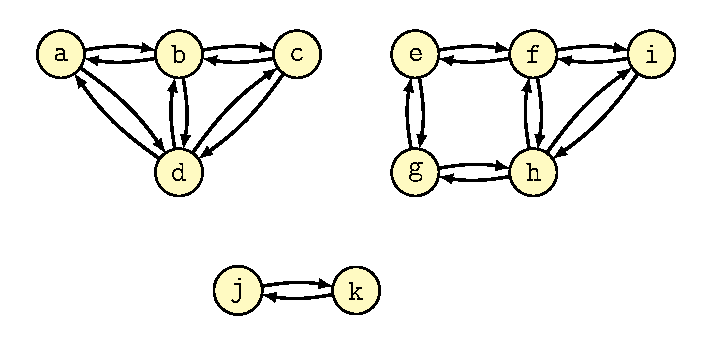
\includegraphics[width=\linewidth, page=1]{ccex-anim-rev}
		\caption{Stato iniziale}
	\end{subfigure}\hfill
	\begin{subfigure}[t]{.48\textwidth}
		\includegraphics[width=\linewidth, page=2]{ccex-anim-rev}
		\caption{Partiamo dal nodo \(a\) per comodità,
			gli assegniamo il valore \(1\)}
	\end{subfigure}

	\begin{subfigure}[t]{.48\textwidth}
		\includegraphics[width=\linewidth, page=7]{ccex-anim-rev}
		\caption{Visito tutti i nodi adiacenti al nodo \(a\)}
	\end{subfigure}\hfill
	\begin{subfigure}[t]{.48\textwidth}
		\includegraphics[width=\linewidth, page=11]{ccex-anim-rev}
		\caption{Una volta arrivati al nodo \(d\) abbiamo già visitato tutti i suoi possibili vicini}
	\end{subfigure}

	\begin{subfigure}[t]{.48\textwidth}
		\includegraphics[width=\linewidth, page=16]{ccex-anim-rev}
		\caption{Abbiamo completato la visita della prima componente connessa}
	\end{subfigure}\hfill
	\begin{subfigure}[t]{.48\textwidth}
		\includegraphics[width=\linewidth, page=17]{ccex-anim-rev}
		\caption{Abbiamo ricontrollato se potevamo ripartire da uno qualsiasi dei nodi della prima componente ma aveva già un \(id\) assegnato, partiamo da \(e\) per comodità}
	\end{subfigure}

	\begin{subfigure}[t]{.48\textwidth}
		\includegraphics[width=\linewidth, page=34]{ccex-anim-rev}
		\caption{Completo così anche la seconda componente\dots}
	\end{subfigure}\hfill
	\begin{subfigure}[t]{.48\textwidth}
		\includegraphics[width=\linewidth, page=35]{ccex-anim-rev}
		\caption{\dots e la terza}
	\end{subfigure}

	\caption{Esempio di identificazione delle componenti connesse\\in un grafo non orientato}
\end{figure}
\clearpage

\section{Verifica ciclicità}

\subsection*{Grafi aciclici non orientati}

\begin{definition}[ciclo, \foreign{cycle}]
In un grafo orientato \(G = (V, E)\), un ciclo \(C\) di lunghezza \(k > 2\) è una sequenza di nodi \(u_0, u_1, \dots u_k\) tale che \((u_i, u_{i+1} \in E)\) (un cammino) per \(0 \leqslant i \leqslant k-1\) e \(u_0 = u_k\) (il primo e l'ultimo nodo coincidono, ossia è chiuso).
\end{definition}

\begin{figure}[H]
	\centering
	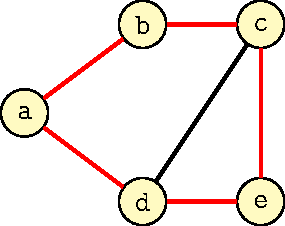
\includegraphics[width=.3\textwidth]{ciclo-non-rev}
	\caption[]{\(k > 2\) esclude cicli banali composti da coppie di archi, i quali sono onnipresenti nei grafi non orientati.
	Questo grafo contine \(3\) cicli, uno di lunghezza \(3\), uno di lunghezza \(4\) ed uno di lunghezza \(5\).}
\end{figure}

\begin{definition}[Grafo aciclico]
Un grafo non orientato che non contiene cicli è detto aciclico.
\end{definition}

\begin{figure}[H]
	\centering
	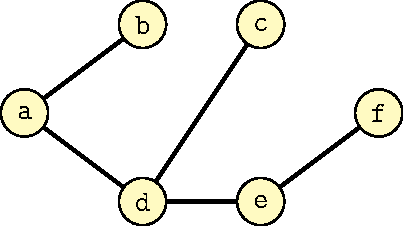
\includegraphics[width=.3\textwidth]{acyclic-und-rev}
	\caption{Un grafo aciclico.}
\end{figure}

Un grafo che contiene cicli è detto \emph{ciclico}, altrimenti viene detto \emph{aciclico}.
Dato un grafo non orientato, vogliamo poter essere in grado di determinare se contiene cicli o meno.
Dobbiamo scrivere quindi un algoritmo che restituisca \True se il grafo contiene un ciclo, \False altrimenti.

\begin{note}
Se è un grafo connesso ed è aciclico, allora è un albero.
\end{note}

L'idea è che se visito un nodo che ho già visitato, allora ho identificato un ciclo.

\clearpage
\begin{algorithm}[H]
	\caption{Ricerca di un ciclo in un grafo non orientato}
	%&../preamble

% arara: pdflatex: { synctex: no }
% arara: latexmk: { clean: partial }
\ifstandalone
\begin{document}
\begin{algorithm}[H]
\fi

\BlankLine
\tcp{restituisce \True se trova un ciclo}
\prototype{\Bool \hasCycleRec{\Graph \(G\), \Node \(u\), \Node \(p\), \Array{\Bool} \(visited\)}}{
	\params{G}[grafo esplorato]
	\params{u}[nodo da esaminare]
	\params{p}[nodo da cui provengo (padre)]
	\params{visited}[vettore dei nodi visitati]

	\BlankLine
	\(visited[u]\) \Assign \True \Comment*[l]{lo visito per la prima volta}

	\BlankLine
	\ForEach(\tcp*[h]{visito tutti i suoi vicini}){\(v \in G.\adj{u} - \{p\}\)}{
		\tcp{\(G.\adj{u} - \{p\}\): non considero il nodo da cui provengo (è un grafo orientato)}

		\BlankLine
		\uIf(\tcp*[h]{ho già visitato il nodo}){\(visited[v]\)}{
			\Return \True \Comment*[l]{ho trovato un ciclo}

			\BlankLine
			\tcp{altrimenti effettuo una visita ricorsiva sul nodo vicino \(v\)}
		}
		\ElseIf{\hasCycleRec{G, v, u, visited}}{
			\tcp{se una qualsiasi delle sottochiamate ritorna vero, allora ho trovato un ciclo}
			\Return \True\;
		}
	}

	\BlankLine
	\tcp{non ho trovato alcun ciclo}
	\Return \False\;
}

\ifstandalone
\end{algorithm}
\end{document}
\fi

	%&../preamble

% arara: pdflatex: { synctex: no }
% arara: latexmk: { clean: partial }
\ifstandalone
\begin{document}
\begin{algorithm}[H]
\fi

\BlankLine
\tcp{ricerca di un ciclo \textbf{per grafi disconnessi}}
\prototype{\Bool \hasCycle{\Graph \(G\)}}{

	\BlankLine
	\Array{\Bool} \(visited\) \Assign \new \Array{\Bool}{1}{G.\setSize} \Comment*[l]{creo il vettore}

	\ForEach(\tcp*[h]{lo inizializzo}){\(u \in G.\VV\)}{
		\(visited[u]\) \Assign \False\;
	}

	\BlankLine
	\ForEach(\tcp*[h]{per ciascun nodo appartenente al grafo}){\(u \in G.\VV\)}{
		\If(\tcp*[h]{il primo nodo non sarà stato visitato}){\Not \(visited[u]\)}{
			\If{\hasCycleRec{G, v, \Null, visited}}{
			\tcp{effettuo una visita ricorsiva sul nodo vicino \(v\)}
				\Return \True\;
			}
		}
	}

	\BlankLine
	\Return \False
}

\ifstandalone
\end{algorithm}
\end{document}
\fi

\end{algorithm}

La parte non ricorsiva dell'algoritmo ci permettere di cercare cicli in grafi non connessi, in quanto stiamo osservando grafi e non alberi (i quali sono connessi).

\clearpage
\subsection*{Grafi aciclici orientati}

Cosa succede se iniziamo a considerare i grafi orientati?

\begin{definition}[ciclo, \foreign{cycle}]
In un grafo non orientato \(G = (V, E)\), un ciclo \(C\) di lunghezza \(k \geqslant 2\) è una sequenza di nodi \(u_0, u_1, \dots u_k\) tale che \((u_i, u_{i+1} \in E)\) (un cammino) per \(0 \leqslant i \leqslant k-1\) e \(u_0 = u_k\) (il primo e l'ultimo nodo coincidono, ossia è chiuso).
\end{definition}

La definizione è identica a parte che ora consideriamo come cicli anche i cammini composti da due soli nodi (\(k \geqslant 2\))

\begin{figure}[H]
	\centering
	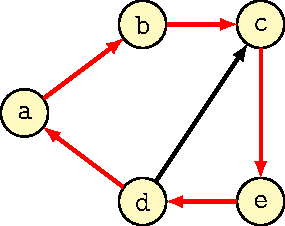
\includegraphics{ciclo-rev}
	\caption[]{\(a, b, c, e, d, a\) è un cammino di lunghezza \(5\)}
\end{figure}

\begin{note}
Un ciclo è detto semplice se tutti i suoi nodi sono distinti (ad esclusione del primo e dell'ultimo)
\end{note}

\begin{definition}[Grafo diretto aciclico, \foreign{Directed Acyclic Graph}]
Un grafo orientato che non contiene cicli è detto DAG (Directed Acyclic Graph)
\end{definition}

\begin{figure}[H]
	\centering
	\begin{subfigure}{.5\textwidth}
		\includegraphics[page=1]{acyclic-rev}
		\caption{Un grafo aciclico.}
	\end{subfigure}\hfill
	\begin{subfigure}{.5\textwidth}
		\includegraphics[page=2]{acyclic-rev}
		\caption{Un grafo ciclico. Il ciclo è dato dai nodi \(c, e, f\).}
	\end{subfigure}
	\caption{Esempio di grafo aciclico e ciclico}
\end{figure}

I \foreign{Directed Acyclic Graph}, DAG d'ora in poi, rappresentano una classe di problemi ben precisi e vedremo degli algoritmi che trattano nello specifico questi grafi.
Il problema è il medesimo: dato un grafo non orientato, vogliamo poter essere in grado di determinare se contiene cicli o meno.
Dobbiamo scrivere quindi un algoritmo che restituisca \True se il grafo contiene un ciclo, \False altrimenti.

L'algoritmo precedente riesce a risolvere anche queto problema?
Riesci a pensare ad un grafo orientato per cui l'algoritmo appena visto non si comporta correttamente?

\begin{figure}[H]
	\centering
	\begin{subfigure}{.18\textwidth}
		\includegraphics[width=\linewidth, page=1]{acyclic-error-rev}
	\end{subfigure}\hfill
	\begin{subfigure}{.18\textwidth}
		\includegraphics[width=\linewidth, page=2]{acyclic-error-rev}
	\end{subfigure}\hfill
	\begin{subfigure}{.18\textwidth}
		\includegraphics[width=\linewidth, page=3]{acyclic-error-rev}
	\end{subfigure}\hfill
	\begin{subfigure}{.18\textwidth}
		\includegraphics[width=\linewidth, page=4]{acyclic-error-rev}
	\end{subfigure}\hfill
	\begin{subfigure}{.18\textwidth}
		\includegraphics[width=\linewidth, page=5]{acyclic-error-rev}
	\end{subfigure}
	\caption[]{Se in un grafo esistono due cammini che portano allo stesso nodo l'algoritmo precedente dirà erroneamente che esiste un ciclo.}
\end{figure}

\clearpage
% NOTE titolo poco esplicativo
% NOTE titolo suggerito: schema di visita in profondità di un grafo
\subsection*{Classificazione degli archi}

Ogni volta che si esamina un arco da un nodo marcato (visitato) ad un nodo non marcato (non visitato), tale arco viene detto arco dell'albero.
Gli archi non inclusi nell'albero possono essere divisi in tre categorie:
\begin{itemize}
	\item se \(u\) è un antenato di \(v\) in \(T\), \((u,v)\) è detto arco in avanti;
	\item se \(u\) è un discendente di \(v\) in \(T\), \((u,v)\) è detto arco all'indietro;
	\item altrimenti viene detto arco di attraversamento.
\end{itemize}

\begin{figure}[H]
	\centering
	\begin{subfigure}{.5\textwidth}\centering
		\includegraphics[page=1]{schema-rev}
		% \caption{}
	\end{subfigure}\hfill
	\begin{subfigure}{.5\textwidth}\centering
		\includegraphics[page=2]{schema-rev}
		% \caption{}
	\end{subfigure}
	% \caption{Esempio di applicazione di \dfsSchema su un grafo semplice}
\end{figure}

\begin{algorithm}[H]
	\caption{Schema per visita dell'albero in profondità}
	%&../preamble

% arara: pdflatex: { synctex: no }
% arara: latexmk: { clean: partial }
\ifstandalone
\begin{document}
\begin{algorithm}[H]
\fi

\BlankLine
\tcp{classifica i lati di un grafo}
\prototype{\dfsSchema{\Graph \(G\), \Node \(u\), \Int {\sffamily\&}\(time\), \Array{\Int} \(dt\), \Array{\Int} \(ft\)}}{

	\params{time}[contatore]
	\params{dt}[tempo di scoperta]
	\params{ft}[tempo di fine]

	\BlankLine
	esamina il nodo \(u\) (caso \emph{pre}-visita)

	\BlankLine
	\Increment{time} \Comment*[l]{incremento il contatore}
	\(dt[u]\) \Assign \(time\) \Comment*[l]{lo memorizzo nel vettore di scoperta}

	\BlankLine
	\tcp{effettuo una visita in profondità}
	\ForEach{\(v \in G.\adj{u}\)}{

		\BlankLine
		\{ \textcolor{black}{esamina l'arco \((u,v)\) (qualsiasi)} \} \Comment*[l]{qui si sviluppa la logica dell'algoritmo}

		\BlankLine
		\uIf(\tcp*[h]{non ho ancora esaminato il nodo}){\(dt[v] \Equal 0\)}{
			\{ \textcolor{arcoAlbero}{esamina l'arco \((u,v)\) (albero)} \}\;

			\BlankLine
			\dfsSchema{G, v, time, dt, ft} \Comment*[l]{effettuo la chiamata ricorsiva}
			\BlankLine

		}
		\uElseIf{\(dt[u] > dt[v]\) \And \(ft[v] \Equal 0\)}{
			\tcp{se raggiungo un mio discendente e non ho ancora terminato la mia visita, allora ho trovato un arco \emph{all'indietro}}
			\{ \textcolor{arcoIndietro}{esamina l'arco \((u,v)\) (indietro)} \}
			\BlankLine

		}
		\uElseIf{\(dt[u] < dt[v]\) \And \(ft[v] \Neq 0\)}{
			\tcp{se raggiungo un mio discendente e ho terminato la mia visita, allora ho trovato un arco \emph{in avanti}}
			\{ \textcolor{arcoAvanti}{esamina l'arco \((u,v)\) (avanti)} \}
			\BlankLine

		}
		\Else{
			\tcp{l'ultimo caso rimanente}
			\{ \textcolor{arcoAttraversamento}{esamina l'arco \((u,v)\) (attraversamento)} \}
		}
	}


	\BlankLine
	\{ visita il nodo \(u\) (\emph{post}-visita) \}

	\BlankLine
	\Increment{time} \tcp{aggiorno il contatore}
	\(ft[u]\) \Assign \(time\) \Comment*[l]{lo memorizzo nel vettore di fine}
}

\ifstandalone
\end{algorithm}
\end{document}
\fi

\end{algorithm}

% \paragraph{Commento}
% La variabile \(time\) è passata per riferimento quindi è globale.
% Inizialmente il suo valore è pari a \(0\), quindi il valore di scoperta assegnato il primo nodo è pari a \(1\).

% \vspace{-20pt}
\begin{figure}[H]

	\begin{subfigure}{.15\textwidth}
		\includegraphics[width=\linewidth, height=3.5cm, keepaspectratio, page=1]{schema-esempio-rev}
	\end{subfigure}\hfill
	\begin{subfigure}{.15\textwidth}
		\includegraphics[width=\linewidth, height=3.5cm, keepaspectratio, page=2]{schema-esempio-rev}
	\end{subfigure}\hfill
	\begin{subfigure}{.15\textwidth}
		\includegraphics[width=\linewidth, height=3.5cm, keepaspectratio, page=3]{schema-esempio-rev}
	\end{subfigure}\hfill
	\begin{subfigure}{.15\textwidth}
		\includegraphics[width=\linewidth, height=3.5cm, keepaspectratio, page=4]{schema-esempio-rev}
	\end{subfigure}\hfill
	\begin{subfigure}{.15\textwidth}
		\includegraphics[width=\linewidth, height=3.5cm, keepaspectratio, page=5]{schema-esempio-rev}
	\end{subfigure}\hfill
	\begin{subfigure}{.15\textwidth}
		\includegraphics[width=\linewidth, height=3.5cm, keepaspectratio, page=6]{schema-esempio-rev}
	\end{subfigure}

	\begin{subfigure}{.15\textwidth}
		\includegraphics[width=\linewidth, height=3.5cm, keepaspectratio, page=7]{schema-esempio-rev}
	\end{subfigure}\hfill
	\begin{subfigure}{.15\textwidth}
		\includegraphics[width=\linewidth, height=3.5cm, keepaspectratio, page=8]{schema-esempio-rev}
	\end{subfigure}\hfill
	\begin{subfigure}{.15\textwidth}
		\includegraphics[width=\linewidth, height=3.5cm, keepaspectratio, page=9]{schema-esempio-rev}
	\end{subfigure}\hfill
	\begin{subfigure}{.15\textwidth}
		\includegraphics[width=\linewidth, height=3.5cm, keepaspectratio, page=10]{schema-esempio-rev}
	\end{subfigure}\hfill
	\begin{subfigure}{.15\textwidth}
		\includegraphics[width=\linewidth, height=3.5cm, keepaspectratio, page=11]{schema-esempio-rev}
	\end{subfigure}\hfill
	\begin{subfigure}{.15\textwidth}
		\includegraphics[width=\linewidth, height=3.5cm, keepaspectratio, page=12]{schema-esempio-rev}
	\end{subfigure}

	\begin{subfigure}{.15\textwidth}
		\includegraphics[width=\linewidth, height=3.5cm, keepaspectratio, page=13]{schema-esempio-rev}
	\end{subfigure}\hfill
	\begin{subfigure}{.15\textwidth}
		\includegraphics[width=\linewidth, height=3.5cm, keepaspectratio, page=14]{schema-esempio-rev}
	\end{subfigure}\hfill
	\begin{subfigure}{.15\textwidth}
		\includegraphics[width=\linewidth, height=3.5cm, keepaspectratio, page=15]{schema-esempio-rev}
	\end{subfigure}\hfill
	\begin{subfigure}{.15\textwidth}
		\includegraphics[width=\linewidth, height=3.5cm, keepaspectratio, page=16]{schema-esempio-rev}
	\end{subfigure}\hfill
	\begin{subfigure}{.15\textwidth}
		\includegraphics[width=\linewidth, height=3.5cm, keepaspectratio, page=17]{schema-esempio-rev}
	\end{subfigure}\hfill
	\begin{subfigure}{.15\textwidth}
		\includegraphics[width=\linewidth, height=3.5cm, keepaspectratio, page=18]{schema-esempio-rev}
	\end{subfigure}

	\caption[]{Visitati in ordine alfabetico per comodità}
\end{figure}

% TODO disegnare lo schema degli intervalli, Gantt chart package?
Osserviamo i numeri assegnati ai nodi; se li consideriamo come intervalli allora \(a \subset b\) perché \([1,8] \subset [2,5]\).
Osservando gli intervalli possiamo quindi dedurre le relazioni di discendenza fra i nodi.

Ma perché li classifichiamo?
Perché possiamo dimostrare delle proprietà sul tipo di archi e usarle per costruire algoritmi migliori.

\begin{theorem*}
Data una visita in profondità di un grafo \(G = (V, E)\), per ogni coppia di nodi \((u, v) \in V\), solo una delle condizioni seguenti è vera:
\begin{itemize}
	\item Gli intervalli \([dt[u], ft[u]\) e \([dt[v], ft[v]]\) sono non-sovrapposti;
	\(u,v\) non sono discendenti l'uno dell'altro nella foresta \foreign{depth-first};
	\item L'intervallo \([dt[u], ft[u]]\) è contenuto in \([dt[v], ft[v]]\);
	\(u\) è un discendente di \(v\) in un albero \foreign{depth-first};
	\item L'intervallo \([dt[v], ft[v]]\) è contenuto in \([dt[u], ft[u]]\);
	\(v\) è un discendente di \(u\) in un albero \foreign{depth-first}.
\end{itemize}
\end{theorem*}

\begin{theorem*}
Un grafo orientato è aciclico se e solo se non esistono archi all'indietro nel grafo
\end{theorem*}

\begin{proof}[Dimostrazione]
Abbiamo due casi:
\begin{enumerate}
	\item se esiste un ciclo, sia \(u\) il primo nodo del ciclo che viene visitato e sia \((u,v)\) un arco del ciclo.
	Il cammino che connette \(u\) a \(v\) verrà prima o poi visitato, e da \(v\) verrà scoperto l'arco all'indietro \((v, u)\) (se esiste un ciclo prima o poi nella visita lo vado a toccare);
	\item se esiste un arco all'indietro \((u,v)\) dove \(v\) è un antenato di \(u\), allora esiste un cammino da \(v\) a \(u\) e un arco da \(u\) a \(v\), ovvero un ciclo.
\end{enumerate}
\end{proof}
Sfruttando questa dimostrazione possiamo quindi semplificare l'algoritmo precedente per la ricerca di un ciclo in un grafo aciclico diretto.

\begin{algorithm}[H]
	\caption{Ricerca di un ciclo in un grafo aciclico diretto}
	%&../preamble

% arara: pdflatex: { synctex: no }
% arara: latexmk: { clean: partial }
\ifstandalone
\begin{document}
\begin{algorithm}[H]
\fi

\BlankLine
\tcp{applicabile solo ai DAG, in quanto non hanno archi all'indietro}
\prototype{\Bool \hasCycle{\Graph \(G\), \Node \(u\), \Int \(\&time\), \Array{\Int} \(dt\), \Array{\Int} \(ft\)}}{
	\tcp{\(u\): il primo nodo che viene visitato}

	\BlankLine
	\Increment{time} \Comment*[l]{aumento il contatore}
	\(dt[u]\) \Assign \(time\) \Comment*[l]{memorizzo il tempo di scoperta}

	\BlankLine
	\ForEach{\(v \in G.\adj{u}\)}{

		\BlankLine
		\uIf(\tcp*[h]{non ho ancora scoperto questo nodo}){\(dt[v] \Equal 0\)}{

			\BlankLine
			\tcp{effettuo una visita ricorsiva}
			\If{\hasCycle{G, v, time, dt, ft}}{
				\Return \True\;
			}
		}

		\BlankLine
		\tcp{logica dell'algoritmo}
		\ElseIf{\(dt[u] > dt[v]\) \And \(ft[v] \Equal 0\)}{
			\tcp{se raggiungo un mio discendente e non ho ancora terminato la mia visita, allora ho trovato un arco \emph{all'indietro} (un ciclo)}
			\Return \True\;
		}
	}

	\BlankLine
	\Increment{time} \Comment*[l]{aumento il contatore}
	\(ft[u]\) \Assign \(time\) \Comment*[l]{memorizzo il tempo di fine}

	\BlankLine
	\tcp{non ho trovato un ciclo}
	\Return \False\;
}

\ifstandalone
\end{algorithm}
\end{document}
\fi

\end{algorithm}

\begin{figure}[H]

	\begin{subfigure}{.20\textwidth}
		\includegraphics[width=\linewidth, page=1]{acyclic-schema-rev}
	\end{subfigure}\hfill
	\begin{subfigure}{.20\textwidth}
		\includegraphics[width=\linewidth, page=2]{acyclic-schema-rev}
	\end{subfigure}\hfill
	\begin{subfigure}{.20\textwidth}
		\includegraphics[width=\linewidth, page=3]{acyclic-schema-rev}
	\end{subfigure}\hfill
	\begin{subfigure}{.20\textwidth}
		\includegraphics[width=\linewidth, page=4]{acyclic-schema-rev}
	\end{subfigure}\hfill
	\begin{subfigure}{.20\textwidth}
		\includegraphics[width=\linewidth, page=5]{acyclic-schema-rev}
	\end{subfigure}

	\begin{subfigure}{.20\textwidth}
		\includegraphics[width=\linewidth, page=6]{acyclic-schema-rev}
	\end{subfigure}\hfill
	\begin{subfigure}{.20\textwidth}
		\includegraphics[width=\linewidth, page=7]{acyclic-schema-rev}
	\end{subfigure}\hfill
	\begin{subfigure}{.20\textwidth}
		\includegraphics[width=\linewidth, page=8]{acyclic-schema-rev}
	\end{subfigure}\hfill
	\begin{subfigure}{.20\textwidth}
		\includegraphics[width=\linewidth, page=9]{acyclic-schema-rev}
	\end{subfigure}\hfill
	\begin{subfigure}{.20\textwidth}
		\includegraphics[width=\linewidth, page=10]{acyclic-schema-rev}
	\end{subfigure}

	\caption[]{Questo è il particolare esempio sulla quale l'algoritmo precedente falliva}
\end{figure}

% TODO aggiunge schema degli intervalli

\begin{note}
Se nello schema degli intervalli ci sono due intervalli sovrapposti, allora esiste un ciclo.
\end{note}

\clearpage
\section{Ordinamento topologico}

L'obiettivo è quello di scrivere un algoritmo che prende in input un DAG e che ne restituisca un possibile ordinamento topologico.

\begin{definition}[ordinamento topologico]
Dato un grafo diretto e aciclico (DAG) \(G\), un ordinamento topologico di \(G\) è un ordinamento lineare dei suoi nodi tale che se \((u,v) \in E\), allora \(u\) appare prima di \(v\) nell'ordinamento.
\end{definition}

\begin{note}
Se il grafo contiene un ciclo, non esiste un ordinamento topologico.
\end{note}

\begin{figure}[H]
	\centering
	\includegraphics[width=.6\textwidth]{top-sort1}
	\caption[Esistenza di più ordinamenti topologici]{Possono esistere più ordinamenti topologici.}
\end{figure}

% L'idea alla base dell'ordinamento topologico
Un approccio banale potrebbe essere il seguente:
\begin{itemize}
	\item trovo un nodo senza archi entranti;
	\item aggiungo questo nodo nell'ordinamento e lo rimuovo dal grafo insieme a tutti i suoi archi;
	\item ripeto questa procedura fino a quando tutti i nodi sono stati rimossi.
\end{itemize}
% TODO grafica esempio banale ordinamento topologico

Si può fare meglio di così.
Eseguiamo una visita in profondità nel quale l'operazione di visita consiste nell'aggiungere il nodo in testa ad una lista in \emph{post}-ordine.
E restituiamo la lista così ottenuta.
Restituiamo in output la sequenza dei nodi ordinati per tempo decrescente di fine.

\begin{figure}[H]

	\begin{subfigure}{.15\textwidth}
		\includegraphics[width=\linewidth, page=1]{topsort-rev}
	\end{subfigure}\hfill
	\begin{subfigure}{.15\textwidth}
		\includegraphics[width=\linewidth, page=2]{topsort-rev}
	\end{subfigure}\hfill
	\begin{subfigure}{.15\textwidth}
		\includegraphics[width=\linewidth, page=3]{topsort-rev}
	\end{subfigure}\hfill
	\begin{subfigure}{.15\textwidth}
		\includegraphics[width=\linewidth, page=4]{topsort-rev}
	\end{subfigure}\hfill
	\begin{subfigure}{.15\textwidth}
		\includegraphics[width=\linewidth, page=5]{topsort-rev}
	\end{subfigure}\hfill
	\begin{subfigure}{.15\textwidth}
		\includegraphics[width=\linewidth, page=6]{topsort-rev}
	\end{subfigure}

	\begin{subfigure}{.15\textwidth}
		\includegraphics[width=\linewidth, page=7]{topsort-rev}
	\end{subfigure}\hfill
	\begin{subfigure}{.15\textwidth}
		\includegraphics[width=\linewidth, page=8]{topsort-rev}
	\end{subfigure}\hfill
	\begin{subfigure}{.15\textwidth}
		\includegraphics[width=\linewidth, page=9]{topsort-rev}
	\end{subfigure}\hfill
	\begin{subfigure}{.15\textwidth}
		\includegraphics[width=\linewidth, page=10]{topsort-rev}
	\end{subfigure}\hfill
	\begin{subfigure}{.15\textwidth}
		\includegraphics[width=\linewidth, page=11]{topsort-rev}
	\end{subfigure}\hfill
	\begin{subfigure}{.15\textwidth}
		\includegraphics[width=\linewidth, page=12]{topsort-rev}
	\end{subfigure}

	\caption{Esempio di ordinamento topologico}

\end{figure}

\begin{algorithm}[H]
	\caption[Ordinamento topologico]{Ordinamento topologico di un grafo orientato aciclico}
	%&../preamble

% arara: pdflatex: { synctex: no }
% arara: latexmk: { clean: partial }
\ifstandalone
\begin{document}
\begin{algorithm}[H]
\fi

\BlankLine
\tcp{ritorna una pila in cui il primo elemento è il primo elemento dell'ordinamento}
\prototype{\Stack \topSort{\Graph \(G\)}}{

	\BlankLine
	\Stack \(S\) \Assign \stackConstructor\;

	\BlankLine
	\Array{\Bool} \(visited\) \Assign \new \Array{\Bool}[1][G.\setSize]

	\ForEach{\(u \in G.\VV\)}{
		\(visited[u]\) \Assign \False\;
	}

	\BlankLine
	\ForEach(\tcp*[h]{per ogni nodo del grafo}){\(u \in G.\VV\)}{

		\If(\tcp*[h]{se non l'ho visitato}){\Not \(visitato[u]\)}{

			\BlankLine
			\tcp{effettua una chiamata ricorsiva}
			\topSortdfs{G, u, visitato, S}
		}
	}

	\BlankLine
	\Return \(S\)\;
}

\ifstandalone
\end{algorithm}
\end{document}
\fi

	%&../preamble

% arara: pdflatex: { synctex: no }
% arara: latexmk: { clean: partial }
\ifstandalone
\begin{document}
\begin{algorithm}[H]
\fi

\BlankLine
\tcp{restituisce l'ordinamento topologico dei nodi di un DAG}
\prototype{\Int \topSortdfs{\Graph \(G\), \Node \(u\), \Array{\Bool} \(visitato\), \Stack \(S\)}}{

	\BlankLine
	\(visitato[u]\) \Assign \True \Comment*[l]{imposta il nodo come visitato}

	\BlankLine
	\ForEach{\(v \in G.\adj{u}\)}{
		\tcp{è una grafo diretto aciclico quindi non ho bisogno di ricordarmi da dove sono venuto}
		\If{\Not \(visitato[v]\)}{

			\BlankLine
			\tcp{effettua una visita in profondità}
			\(i\) \Assign \topSortdfs{G, u, visitato, S}\;
		}
	}

	\BlankLine
	\(S.\stackPush{u}\) \Comment*[l]{aggiungi il nodo in testa alla pila}
}


\ifstandalone
\end{algorithm}
\end{document}
\fi

\end{algorithm}

Quando termino tutte le chiamate ricorsive l'algoritmo restituisce un ordinamento topologico dei nodi del grafo dato in input; quando un nodo è \enquote{finito} tutti i suoi discendenti sono stati scoperti e aggiunti alla lista.
Aggiungendolo in testa alla lista, il nodo si trova prima dei nodi a cui i suoi archi puntano, ossia i suoi discendenti.

\begin{figure}[H]

	\begin{subfigure}{.15\textwidth}
		\includegraphics[width=\linewidth, height=4.5cm, keepaspectratio, page=7]{topsort-rev}
	\end{subfigure}\hfill
	\begin{subfigure}{.15\textwidth}
		\includegraphics[width=\linewidth, height=4.5cm, keepaspectratio, page=8]{topsort-rev}
	\end{subfigure}\hfill
	\begin{subfigure}{.15\textwidth}
		\includegraphics[width=\linewidth, height=4.5cm, keepaspectratio, page=9]{topsort-rev}
	\end{subfigure}\hfill
	\begin{subfigure}{.15\textwidth}
		\includegraphics[width=\linewidth, height=4.5cm, keepaspectratio, page=10]{topsort-rev}
	\end{subfigure}\hfill
	\begin{subfigure}{.15\textwidth}
		\includegraphics[width=\linewidth, height=4.5cm, keepaspectratio, page=11]{topsort-rev}
	\end{subfigure}\hfill
	\begin{subfigure}{.15\textwidth}
		\includegraphics[width=\linewidth, height=4.5cm, keepaspectratio, page=12]{topsort-rev}
	\end{subfigure}

	\caption[Esempio di ordinamento topologico alternativo]{Esempio di ordinamento topologico alternativo al precendente,\\il quale dimostra informalmente che l'algoritmo funziona partendo da qualsiasi nodo}

\end{figure}

\clearpage
\section{Componenti fortemente connesse}

\begin{definition}[Grafo fortemente connesso]
Un grafo orientato \(G = (V,E)\) è \alert{fortemente connesso} se e solo se ogni suo nodo è raggiungibile da ogni altro suo nodo.
\end{definition}

\begin{definition}[Componente fortemente connessa]
Un grafo \(G' = (V',E')\) è una \alert{componente fortemente connessa} di \(G\) se e solo se \(G'\) è un sottografo connesso e massimale di \(G\).
\end{definition}

Le definizioni di fortemente connessa è identica alla definizione di componente connessa, ma si opera su grafi orientati, mentre prima operavamo su grafi non orientati.

\begin{figure}[H]
	\centering
	\hfill
	\begin{subfigure}{.4\textwidth}
		\includegraphics[width=\linewidth, page=1]{scc}
	\end{subfigure}\hfill
	\begin{subfigure}{.4\textwidth}
		\includegraphics[width=\linewidth, page=2]{scc}
	\end{subfigure}
	\hfill\null
	\caption[Identificazione della componente fortemente connessa]{\((a)\) e \((b)\) sono componenti connesse massimali, \((c, d, e, f)\) è una componente fortemente connessa.}
\end{figure}

Per definire le componenti fortemente connesse potremmo applicare l'algoritmo \ConnectedComponents; purtroppo il risultato dipende dal nodo di partenza.

\begin{figure}[H]
	\centering
	\begin{subfigure}{.3\textwidth}
		\includegraphics[width=\linewidth, page=3]{scc}
	\end{subfigure}\hfill
	\begin{subfigure}{.3\textwidth}
		\includegraphics[width=\linewidth, page=4]{scc}
	\end{subfigure}\hfill
	\begin{subfigure}{.3\textwidth}
		\includegraphics[width=\linewidth, page=5]{scc}
	\end{subfigure}
	\caption[]{Il risultato dipende dal nodo di partenza.}
\end{figure}

\clearpage
\subsection{L'algoritmo di Kosaraju}

L'algoritmo di Kosaraju:
\begin{enumerate}
	\item effettua una visita in profondità del grafo \(G\)
	\item ne calcola il grafo trasposto \(G^T\) (ossia il grafo con la direzione degli archi invertiti)
	\item esegue una visita in profondità sul grafo trasposto \(G^T\) utilizzando l'algoritmo \ConnectedComponents, esaminando i nodi nell'ordine inverso di tempo di fine della prima visita;
\end{enumerate}
Le componenti connesse (e i relativi alberi \foreign{depth-first}) rappresentano le componenti fortemente connesse \mbox{di \(G\)}.

\begin{algorithm}[H]
	\caption{Algoritmo di Kosaraju}
	%&../preamble

% arara: pdflatex: { synctex: no }
% arara: latexmk: { clean: partial }
\ifstandalone
\begin{document}
\begin{algorithm}[H]
\fi

\BlankLine
\tcp{indentifica le componenti fortemente connesse}
\prototype{\Array{\Int} \StrongConnectedComponents{\Graph G}}{

	\BlankLine
	\Stack \(S\) \Assign \topSort{\(G\)} \Comment*[l]{prima visita}
	\(G^T\) \Assign \transpose{\(G\)} \Comment*[l]{trasposizione del grafo}

	\BlankLine
	\Return \ConnectedComponents{\(G^T, S\)} \Comment*[l]{seconda visita}
}

\ifstandalone
\end{algorithm}
\end{document}
\fi

\end{algorithm}

Restituisce un vettore di interi che associa ad ogni nodo l'id della sua componente fortemente connessa.
Applicando l'algoritmo di ordinamento topologico \emph{su un grafo generale}, siamo sicuri che:
\begin{itemize}
	\item se un arco \((u,v)\) non appartiene ad un ciclo, allora \(u\) viene listato prima di \(v\) nella sequenza ordinata;
	\item gli archi di un ciclo vengono listati in qualche ordine (che è ininfluente).
\end{itemize}
Utilizziamo quindi la procedura \topSort per ottenere i nodi in ordine decrescente di tempo di fine.

Nella \topSort non calcoliamo nemmeno i tempi di fine, li utilizziamo semplicemente per dimostrare che i nodi vengono ordinati in ordine inverso di tempo di fine.

% \caption{esempi di esecuzione di ordinamento topologico, partenza dal nodo \(a\)}

\begin{definition}[Grafo trasposto]
Dato un grafo orientato \(G = (V, E)\), il grafo trasposto \mbox{\(G_t = (V,E_T)\)} ha gli stessi nodi e gli archi orientati in senso opposto: \(E_T = \{ (u,v) \mid (v,u) \in E \}\)
\end{definition}

\begin{algorithm}[H]
	\caption{Calcolo del grafo trasposto}
	%&../preamble

% arara: pdflatex: { synctex: no }
% arara: latexmk: { clean: partial }
\ifstandalone
\begin{document}
\begin{algorithm}[H]
\fi

\BlankLine
\tcp{restituisce il grafo transposto}
\prototype{\Array{\Int} \transpose{\Graph \(G\)}}{

	\BlankLine
	\Graph \(G^T\) \Assign \graphConstructor \Comment*[l]{creo il grafo}

	\BlankLine
	\ForEach{\(u \in G.\VV\)}{
		\(G^T\).\nodeInsert{\(u\)} \Comment*[l]{aggiungo gli stessi nodi}
	}

	\BlankLine
	\ForEach{\(u \in G.\VV\)}{
		\ForEach{\(v \in G.\adj{u}\)}{
			\(G^T\).\edgeInsert{\(v,u\)} \Comment*[l]{li aggiungo in ordine inverso}
		}
	}

	\BlankLine
	\tcp{restituisco il grafo trasposto}
	\Return \(G^T\)\;
}

\ifstandalone
\end{algorithm}
\end{document}
\fi

\end{algorithm}

\clearpage
\paragraph{Complessità}
Il costo computazionale totale ammonta a \(\Omicron(m+n)\), in quanto aggiungere i nodi costa \(\Omicron(n)\), gli archi \(\Omicron(m)\) ed ogni operazione costa \(\Omicron(1)\).

\begin{figure}[H]
	\begin{subfigure}{.5\textwidth}
		\includegraphics[width=\linewidth, page=2]{scc3}
		\caption{Grafo originale}
	\end{subfigure}\hfill
	\begin{subfigure}{.5\textwidth}
		\includegraphics[width=\linewidth, page=3]{scc3}
		\caption{Grafo trasposto}
	\end{subfigure}
\end{figure}

\begin{algorithm}[H]
	\caption{Identificazione delle componenti connesse alternativa}
	%&../preamble

% arara: pdflatex: { synctex: no }
% arara: latexmk: { clean: partial }
\ifstandalone
\begin{document}
\begin{algorithm}[H]
\fi

\BlankLine
% \tcp{identifica le componenti connesse di un grafo non orientato}
\tcp{parte iterativa}
\prototype{\Array{\Int} \ConnectedComponents{\Graph G, \Stack S}}{

	\BlankLine
	\tcp{creo un vettore della dimensione dei nodi del grafo}
	\Array{\Int} \(id\) \Assign \new \Array{\Int}[1][G.\setSize]\;
	\tcp{inizializzo il vettore}
	\ForEach{\(u \in G.\VV\)}{
		\(id[u] \Assign 0\)\;
	}
	\tcp{contatore delle componenti connesse}
	\Int \(counter \Assign 0\)\;

	\BlankLine
	\While(\tcp*[h]{fintanto che la pila non è vuota}){\alert{\Not \(S.\stackEmpty\)}}{

		\alert{\(u\) \Assign \(S\).\stackPop}\;

		\BlankLine
		\If(\tcp*[h]{ho trovato una nuova componente connessa}){\(id[u] \Equal 0\)}{
			\Increment{counter} \Comment*[l]{aggiorno il contatore}

			\BlankLine
			\tcp{effettuo una chiamata ricorsiva sul nodo scoperto}
			\ccdfs{G, counter, u, id}
		}
	}

	\BlankLine
	\tcp{restituisco l'identificativo della componente connessa}
	\Return \(id\)
}
\ifstandalone
\end{algorithm}
\end{document}
\fi

	%&../preamble

% arara: pdflatex: { synctex: no }
% arara: latexmk: { clean: partial }
\ifstandalone
\begin{document}
\begin{algorithm}[H]
\fi

\BlankLine
\tcp{visita ricorsiva di ciascuna componente}
\prototype{\ccdfs{\Graph G, \Int counter, \Node u, \Array{\Int} id}}{

	\vspace{2pt}
	\params{counter}[identificatore di quante cc ho trovato fin'ora]
	\params{u}[il nodo che sto visitando]
	\params{id}[l'identificativo della componente]

	\BlankLine
	\tcp{memorizzo l'identificativo della cc}
	\(id[v] \Assign counter\)\;

	\BlankLine
	\ForEach(\tcp*[h]{per ciascun nodo adiacente}){\(v \in G.\adj{u}\)}{

		\BlankLine
		\If(\tcp*[h]{non è ancora stato visitato}){\(id[v] \Equal 0\)}{
			\tcp{\(v\): il nodo su cui vado ad operare}

			\BlankLine
			\ccdfs{G, counter, v, id} \Comment*[l]{lo visito ricorsivamente}
		}
	}
}
\ifstandalone
\end{algorithm}
\end{document}
\fi

\end{algorithm}

Invece di esaminare i nodi in ordine arbitrario, questa versione di \ConnectedComponents li esamina nell'ordine \textsc{LIFO} memorizzato nello stack.

\begin{figure}[H]\centering
	\includegraphics[page=4]{scc3}
	\caption[Identificazione delle componenti fortemente connesse]{Identificazione delle componenti fortemente connesse;\\l'ordine in cui li visito è quello della pila \texttt{\{ a, b, c, e, d, f \} }}
\end{figure}

\begin{algorithm}[H]
	\caption{Identificazione delle componenti fortemente connesse}
	%&../preamble

% arara: pdflatex: { synctex: no }
% arara: latexmk: { clean: partial }
\ifstandalone
\begin{document}
\begin{algorithm}[H]
\fi

\BlankLine
\tcp{indentifica le componenti fortemente connesse}
\prototype{\Array{\Int} \StrongConnectedComponents{\Graph G}}{

	\BlankLine
	\Stack \(S\) \Assign \topSort{\(G\)} \Comment*[l]{prima visita}
	\(G^T\) \Assign \transpose{\(G\)} \Comment*[l]{trasposizione del grafo}

	\BlankLine
	\Return \ConnectedComponents{\(G^T, S\)} \Comment*[l]{seconda visita}
}

\ifstandalone
\end{algorithm}
\end{document}
\fi

\end{algorithm}

\paragraph{Complessità}
Ognuna delle fasi che compongono l'algoritmo:
\begin{enumerate}
	\item visita in profondità della \topSort;
	\item la trasposizione del grafo di \transpose;
	\item la visita delle componenti connesse.
\end{enumerate}
richiede un costo di \(\Omicron(m+n)\).
Quindi la complessità è lineare nel numero di nodi e nel numero di archi, ossia \(\Omicron(m+n)\).

\begin{figure}[H]\centering
	\begin{subfigure}[t]{.3\textwidth}
		\includegraphics[width=\linewidth, page=1]{scc4}
		\caption{La prima visita parte da \(f\),\\la seconda dal nodo \(a\)}
	\end{subfigure}\hfill
	\begin{subfigure}[t]{.3\textwidth}
		\includegraphics[width=\linewidth, page=3]{scc4}
		\caption{Calcolo il grafo trasposto \(G^T\)}
	\end{subfigure}\hfill
	\begin{subfigure}[t]{.3\textwidth}
		\includegraphics[width=\linewidth, page=4]{scc4}
		\caption{Identificazione delle componenti fortemente connesse}
	\end{subfigure}
	\caption[]{Una seconda esecuzione dell'ordinamento topologico}
\end{figure}

\clearpage
\subsection{Dimostrazione di correttezza}

\begin{definition}[Grafo delle componenti]
Il grafo delle componenti si definisce come il grafo \(C(G) = (V_c, E_c)\), dove:
\begin{itemize}
	\item \(V_c = \{C_1, C_2, \dots, C_k\}\), dove \(C_i\) è la \(i\)-esima componente fortemente connessa del grafo \(G\);
	\item \(E_c = \{(C_i, C_j) \mid \exists (u_i, v_i) \in E \,\colon u_i \in C_i \land u_j \in C_j\}\)
\end{itemize}
\end{definition}

\begin{figure}[H]
	\hfill
	\begin{subfigure}{.4\textwidth}
		\includegraphics[width=\linewidth, page=1]{scc2}
		\caption{Grafo delle componenti del grafo}
	\end{subfigure}\hfill
	\begin{subfigure}{.4\textwidth}
		\includegraphics[width=\linewidth, page=6]{scc2}
		\caption{Grafo delle componenti del grafo trasposto}
	\end{subfigure}
	\hfill\null
	\caption[Grafo delle componenti del grafo e del grafo trasposto]{}
\end{figure}

% La relazione che intercorre
Quando si traspone un grafo fortemente connesso, l'insieme di nodi che compongono il grafo delle componenti connesse rimane lo stesso, mentre gli archi sono in direzione inversa.

\begin{note}
Il grafo delle componenti è aciclico poiché se contenesse un ciclo, il ciclo stesso sarebbe una più grande componente fortemente connessa, il che è assurdo.
\end{note}

Se il grafo delle componenti è aciclico, allora posso farne un'ordinamento topologico.
Possiamo definire quindi \(dt(C) = \minFunction\{dt(u) \mid u \in C\}\) e \(ft(C) = \maxFunction\{ft(u) \mid u \in C\}\), i quali corrisponderanno ai tempo di inizio e di fine del primo nodo visitato in \(C\).

\begin{theorem*}
Siano \(C\) e \(C'\) due distinte componenti fortemente connesse nel grafo orientato \mbox{\(G = (V,E)\)}.
Se c'è un arco \((C, C') \in E_c\), allora \(ft(C) > ft(C')\).
\end{theorem*}

La componente che finisce la visita per ultima è la componente dalla quale si possono raggiungere le altre componenti.

\begin{figure}[H]
	\begin{subfigure}{.5\textwidth}
		\includegraphics[width=\linewidth, page=3]{scc2}
		\caption{Grafo delle componenti del grafo}
	\end{subfigure}\hfill
	\begin{subfigure}{.5\textwidth}
		\includegraphics[width=\linewidth, page=4]{scc2}
		\caption{Grafo delle componenti del grafo trasposto}
	\end{subfigure}
\end{figure}

\begin{corollario*}
Siano \(C_u\) e \(C_v\) due componenti fortemente connesse distinte del grafo orientato \(G = (V,E)\).
Se c'è un arco \((u,v) \in E_t\) tale che \(u \in C_u\) e \(v \in C_v\), allora \(ft(C_u) < ft(C_v)\).
\end{corollario*}

In generale:
\[(u,v) \in E_t \Rightarrow (v,u) \in E \Rightarrow (C_v, C_u) \in E_c \Rightarrow ft(C_v) > ft(C_u) \Rightarrow ft(C_u) < ft(C_v)\]
Nel nostro caso:
\[(b,a) \in E_t \Rightarrow (a,b) \in E \Rightarrow (C_a, C_b) \in E_c \Rightarrow \underset{12}{ft(C_a)} > \underset{11}{ft(C_b)} \Rightarrow \underset{11}{ft(C_b)} < \underset{12}{ft(C_a)}\]

Se la componente \(C_u\) e la componente \(C_v\) sono connesse da un arco \((u,v) \in E_t\), allora possiamo dedurne che \(ft(C_u) < ft(C_v)\) (dal corollario) e che la visita di \(C_v\) inizierà prima della visita di \(C_u\) (dal teorema).
Non esistendo cammini fra \(C_v\) e \(C_u\) in \(G_t\) (altrimenti il grafo sarebbe ciclico) la visita di \(C_v\) non raggiungerà \(C_u\).
In altre parole, l'algoritmo \ConnectedComponents assegnerà correttamente gli indentificatori delle componenti ai nodi.

\subsection*{Algoritmo di Tarjan}

L'algoritmo di Tarjan è preferito a quello di Kosaraju il quale, avendo comunque la medesima complessità computazionale (\(\Omicron(m+n)\)), è preferito a quest'ultimo in quanto necessita di una sola visita e non richiede la trasposizione del grafo (al posto di una doppia visita e di memoria aggiuntiva).

\subsection*{Applicazioni}

Gli algoritmi sulle componenti fortemente connesse possono essere utilizzati per risolvere il problema \enquote{2-satisfiability} (2-SAT), un problema di soddisfacibilità booleana con clausole composte da coppie di letterali.

\ifsubfile
\end{document}
\fi
